%% Copernicus Publications Manuscript Preparation Template for LaTeX Submissions
%% ---------------------------------
%% This template should be used for copernicus.cls
%% The class file and some style files are bundled in the Copernicus Latex Package, which can be downloaded from the different journal webpages.
%% For further assistance please contact Copernicus Publications at: production@copernicus.org
%% https://publications.copernicus.org/for_authors/manuscript_preparation.html

%% copernicus_rticles_template (flag for rticles template detection - do not remove!)

%% Please use the following documentclass and journal abbreviations for discussion papers and final revised papers.

%% 2-column papers and discussion papers
\documentclass[gc, manuscript]{copernicus}



%% Journal abbreviations (please use the same for preprints and final revised papers)

% Advances in Geosciences (adgeo)
% Advances in Radio Science (ars)
% Advances in Science and Research (asr)
% Advances in Statistical Climatology, Meteorology and Oceanography (ascmo)
% Annales Geophysicae (angeo)
% Archives Animal Breeding (aab)
% Atmospheric Chemistry and Physics (acp)
% Atmospheric Measurement Techniques (amt)
% Biogeosciences (bg)
% Climate of the Past (cp)
% DEUQUA Special Publications (deuquasp)
% Drinking Water Engineering and Science (dwes)
% Earth Surface Dynamics (esurf)
% Earth System Dynamics (esd)
% Earth System Science Data (essd)
% E&G Quaternary Science Journal (egqsj)
% EGUsphere (egusphere) | This is only for EGUsphere preprints submitted without relation to an EGU journal.
% European Journal of Mineralogy (ejm)
% Fossil Record (fr)
% Geochronology (gchron)
% Geographica Helvetica (gh)
% Geoscience Communication (gc)
% Geoscientific Instrumentation, Methods and Data Systems (gi)
% Geoscientific Model Development (gmd)
% History of Geo- and Space Sciences (hgss)
% Hydrology and Earth System Sciences (hess)
% Journal of Bone and Joint Infection (jbji)
% Journal of Micropalaeontology (jm)
% Journal of Sensors and Sensor Systems (jsss)
% Magnetic Resonance (mr)
% Mechanical Sciences (ms)
% Natural Hazards and Earth System Sciences (nhess)
% Nonlinear Processes in Geophysics (npg)
% Ocean Science (os)
% Polarforschung - Journal of the German Society for Polar Research (polf)
% Primate Biology (pb)
% Proceedings of the International Association of Hydrological Sciences (piahs)
% Safety of Nuclear Waste Disposal (sand)
% Scientific Drilling (sd)
% SOIL (soil)
% Solid Earth (se)
% The Cryosphere (tc)
% Weather and Climate Dynamics (wcd)
% Web Ecology (we)
% Wind Energy Science (wes)

% Pandoc citation processing

% The "Technical instructions for LaTex" by Copernicus require _not_ to insert any additional packages.
% 
% tightlist command for lists without linebreak
\providecommand{\tightlist}{%
  \setlength{\itemsep}{0pt}\setlength{\parskip}{0pt}}


%
\begin{document}


\title{New insights into the Weddell Sea ecosystem applying a network
approach}


\Author[1, *]{Tomás I.}{Marina}
\Author[1, *]{Leonardo A.}{Saravia}
\Author[2]{Susanne}{Kortsch}


\affil[1]{Centro Austral de Investigaciones Científicas (CADIC-CONICET),
Ushuaia, Argentina}
\affil[2]{University of Helsinki, Helsinki, Finland}
\affil[*]{These authors contributed equally to this work.}

\runningtitle{New insights into the Weddell Sea food web}

\runningauthor{Marina et al.}

\correspondence{Tomás I. Marina (tomasimarina@gmail.com) and Leonardo A.
Saravia (arysar@gmail.com)}


\received{}
\pubdiscuss{} %% only important for two-stage journals
\revised{}
\accepted{}
\published{}

%% These dates will be inserted by Copernicus Publications during the typesetting process.


\firstpage{1}

\maketitle


\begin{abstract}
The abstract goes here. It can also be on \emph{multiple lines}.
\end{abstract}




\introduction[Introduction]

Introduction text goes here.

The objective of this work was twofold: 1) estimate the strength for
each interaction in the Weddell Sea food web, and 2) determine key
trophic species considering weighted and unweighted properties and the
influence on the stability of the network.

\section{Methodology}

\subsection{Study area}

The high Antarctic Weddell Sea shelf is situated between 74 and 78ºS
with a length of approximately 450 km (Figure 1). Water depth varies
from 200 to 500 m. Shallower areas are covered by continental ice, which
forms the coastline along the eastern and southern part of the Weddell
Sea. The shelf area contains a complex three-dimensional habitat with
large biomass, intermediate to high diversity in comparison to benthic
boreal communities and a spatially patchy distribution of organisms
\citep{Dayton1990, Teixido2002}.

\begin{figure}
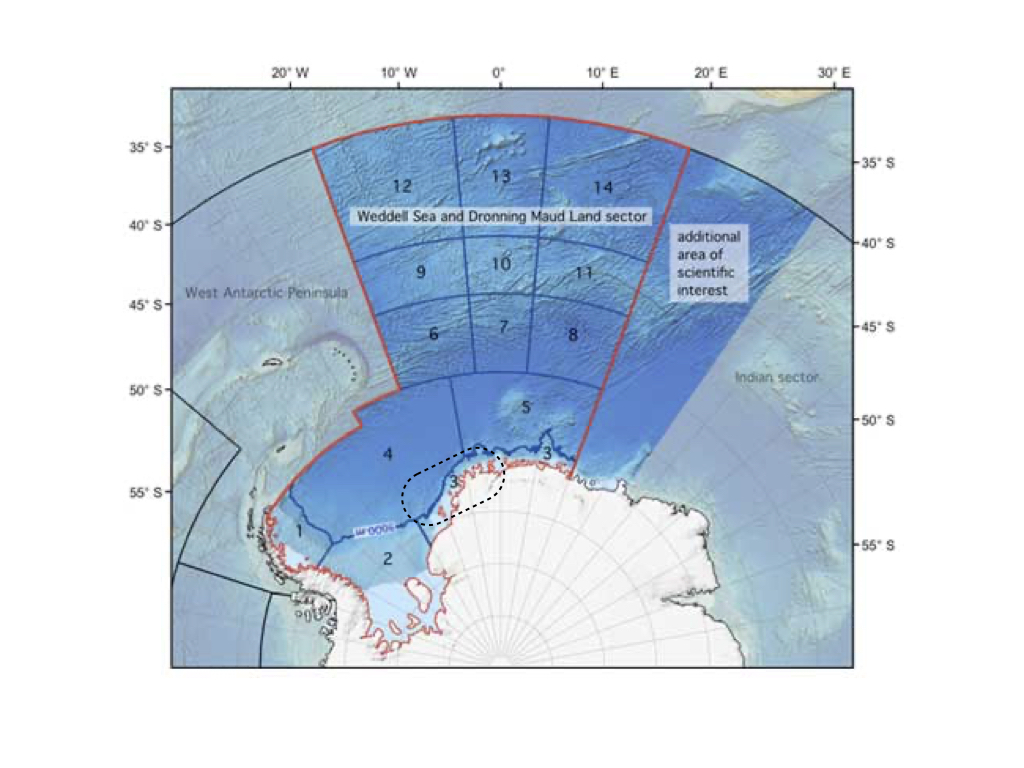
\includegraphics[width=12cm]{WeddellSea_map} \caption{Map of the Weddell Sea and Dronning Maud Land sector highlighting the high Antarctic shelf as a dashed-line contour. Modified from www.soos.aq.}\label{fig:unnamed-chunk-1}
\end{figure}

\subsection{Weddell Sea food web dataset}

We obtained the dataset of the Weddell Sea food web from the GlobAL
daTabasE of traits and food Web Architecture (GATEWAy, version 1.0) of
the German Centre for Integrative Biodiversity Research (iDiv)
Halle-Jena-Leipzig \citep{Brose2018}. This open access database is a
list of predator-prey interactions that contains several highly-resolved
food webs, including biological data about the consumer and resource
species involved in each trophic interaction (i.e.~mean mass).
Furthermore, it incorporates information on the interaction itself, such
as the dimensionality.

This marine food web compiles all the food web data available for the
high Antarctic Weddell Sea collected since 1983, and is one of the most
highly-resolved marine food webs documented to date. It's noteworthy
that it is a summary network that ignores seasonal changes
\citep{Jacob2011}.

\subsection{Dataset analyses}

We analysed the food web of the Weddell Sea by: a) estimating the
strength of each interaction; b) studying the properties of the species
in a network approach; and c) comparing the stability of the food web
after performing extinction simulations.

\subsubsection{Interaction strength estimation and distribution}

To estimate the strength of each interaction in the food web, we
followed the methodology proposed by \citet{Pawar2012}. The minimum data
requirements are: body mass of the consumer (predator) and resource
(prey), and the interaction dimensionality classified as 2 or 3
dimensions. GATEWAy v.1.0 does provide information on the mean mass for
consumers and resources (except for `detritus' and `sediment') for every
interaction, but lacks the dimensionality for 924 interactions. To solve
this issue, we used the information about movement type for consumer and
resource. Then, we classified the interaction as 2D when both consumer
and resource move in 2D (e.g., both are sessile or walking) or if a
consumer moves in 3D and a resource in 2D (e.g., swimming consumer and
sessile/walking resource). The interaction was classified as 3D when
both consumer and resource move in 3D (e.g., both swimming) or if the
consumer moves in 2D and resource in 3D (e.g., sessile/walking consumer,
swimming resource) \citep{Pawar2012}.

The main equation we used for estimating the interaction strength IS is:

\begin{equation}
IS = \alpha x_R \frac{m_R}{m_C}
\end{equation}

where \vec{\alpha} is the search rate, \vec{x_R} is the density of the
resource, and \vec{m_R} and \vec{m_C} are the body mass of the resource
and the consumer, respectively \citep{Pawar2012}.

We obtained estimations for the resource density and the search rate
from the scaling relationships with the resource and the consumer mass,
respectively (\citet{Pawar2012}). The coefficients of such
relationships, determined by ordinary least squares regression, vary
with the interaction dimensionality. On one hand, resource density
scales with resource mass as a power-law with exponents
\vec{p = -0.79 \pm 0.09} in 2D and \vec{p = -0.86 \pm 0.06} in 3D. Since
mean mass for resources `detritus' and `sediment' were not available in
GATEWAy v.1.0, we calculated it considering the scaling relationship
with consumer mass, also different in 2D and 3D (for details see
equation S9 and figures 2c-d of Supplementary Information in
\citet{Pawar2012}). On the other hand, search rate scales with consumer
mass as a power-law with exponents \vec{p = 0.68 \pm 0.12} in 2D and
\vec{p = 1.05 \pm 0.08} in 3D.

Finally, we fit the distribution of the interaction strengths of the
food web considering six candidate models (Uniform, Normal, Exponential,
Power-law, log-Normal and Gamma) using maximum likelihood
\citep{McCallum2008}, and selected the model performance by computing
the Akaike Information Criterion \citep{Burnham2002}.

\subsubsection{Species properties}

In order to individually characterize the species of the food web, we
considered weighted and unweighted properties (Figure 2). The former is
based on the estimation of the interaction strength described in the
previous section. The latter is related to properties commonly used in
qualitative (presence/absence of interaction) food web studies
\citep{Martinez1991, Dunne2002, Borrelli2014}.

As weighted property we took into account the mean interaction strength,
meaning the average strength of all interactions. After exploring the
distribution of the interaction strength among the species of the food
web, we decided to apply the k-means clustering method, which aims to
partition the species into k groups such that the sum of squares from
points to the assigned cluster centres is minimized
\citep{Hartigan1979}.

As unweighted properties we used: a) degree or the total number of
trophic interactions, taking into account in- and out-interactions (role
as predator and prey, respectively); b) trophic level or the position in
the food web relative to primary producers/detritus; and c) trophic
similarity or the trophic overlap between species based on shared and
unique resources and consumers.

Formulas used to obtain the mentioned species properties are described
in Appendix A1.

\begin{figure}
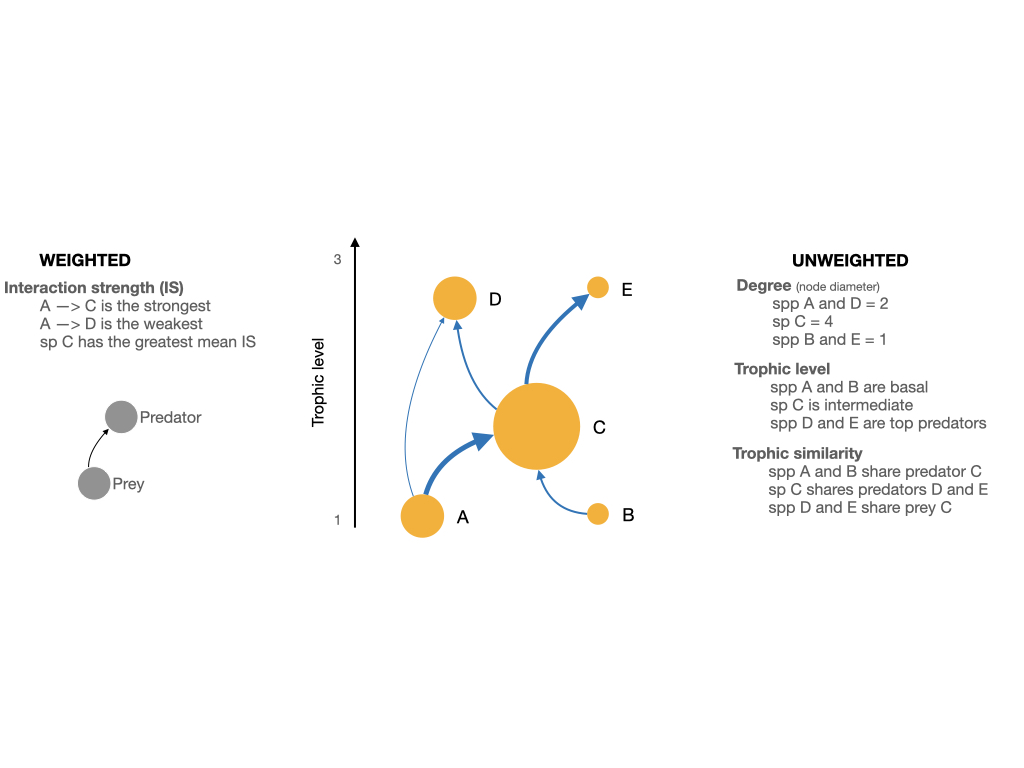
\includegraphics[width=12cm]{ToyFoodWeb} \caption{Scheme of a network showing the weighted and unweighted properties we used to characterize the species of the Weddell Sea food web.}\label{fig:unnamed-chunk-2}
\end{figure}

\subsubsection{Stability and extinction simulations}

Finally, we run extinction simulations and estimated its impact on the
stability of the network. For this, we calculated a stability index
called Quasi-Sign Stability (QSS), which is the proportion of stable
networks using randomized Jacobians and keeping the predator-prey sign
structure fixed \citep{Allesina2008}. With the aim of analysing the
effect of each species on the food web's stability, we deleted one
species at a time, so the network size was reduced by one. After each
species extinction, we calculated the QSS for the food web minus one
species (size = 489) and compared it with the QSS for the whole network
(size = 490); we performed 1000 simulations for each species. Then we
statistically analysed such difference with an Anderson-Darling test
\citep{Scholz1987}. The formula for the QSS is described in Appendix A2.

All analyses were performed in R software, mainly using packages igraph
\citep{Csardi2005}, cheddar \citep{Hudson2013}, and multiweb
\citep{Saravia2019}. The source code and data are available at
https://github.com/EcoComplex/WeddellSea.

\section{Results}

\subsection{Interaction strength}

In this work we have estimated the interaction strength for the most
highly-resolved marine food web to date, which comprises 490 species and
16041 predator-prey interactions (Figure 3).

\begin{figure}
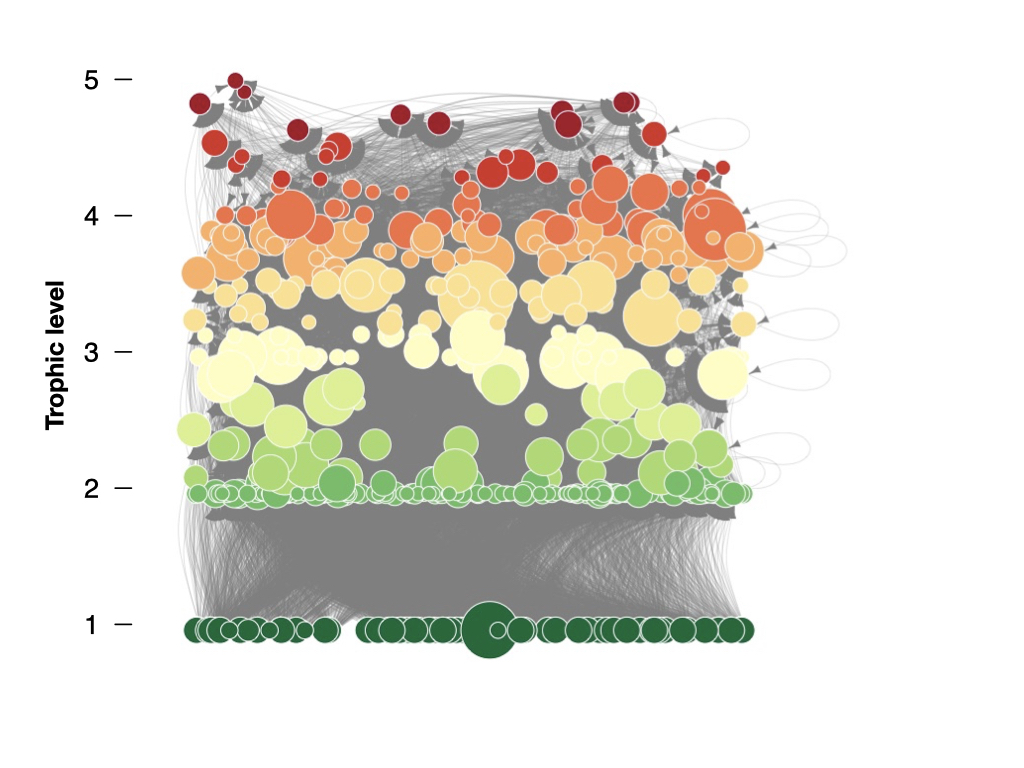
\includegraphics[width=12cm]{WeddellSea_net} \caption{Graphic representation of the Weddell Sea food web. Species (nodes) are arranged verticaly and colored by trophic level. The diameter of the node indicates the total number of interactions. Predator-prey interactions are represented by the arrows, from the prey to the predator.}\label{fig:unnamed-chunk-3}
\end{figure}

The distribution of the interaction strength best fit to a log-Normal
model, which indicates that there is a prevalent skew towards weaker
interactions (Figure 4, Table 1). Regarding the distribution of the mean
interaction strength among the species of the food web, the clustering
method shows that species can be classified in two groups: `High' and
`Low' interaction strength.

\begin{figure}
\includegraphics[width=12cm]{IS_dist} \caption{Frequency distribution of interaction strengths for the Weddell Sea food web (n = 490).}\label{fig:unnamed-chunk-4}
\end{figure}

\begin{table}[t]
\caption{Model comparison (AIC) for the distribution of interaction strengths of the Weddell Sea food web.}
\begin{tabular}{l c c c}
\tophline

Model & df & AIC & deltaAIC \\
\middlehline
log-Normal & 2 & -356579 & 0 \\
\middlehline
Gamma & 2 & -352575 & 4004 \\
\middlehline
Power-law & 2 & -347646 & 8933 \\
\middlehline
Exponential & 1 & -262852 & 93726 \\
\middlehline
Normal & 2 & -222785 & 133793 \\
\middlehline
Uniform & 2 & -178001 & 178578 \\

\bottomhline
\end{tabular}
\end{table}

\subsection{Species properties and stability}

Clustering in 2 groups: high and low IS Linear regressions btw IS
(weighted) and unweighted prop. Biplots btw QSS difference and weighted
and unweighted prop.

\section{Discussion}

``Low functional redundancy at key trophic levels makes these ecosystems
(polar pelagic) particularly sensitive to change''. \citep{Murphy2016}

\section{Examples from the official template}

\subsection{FIGURES}

When figures and tables are placed at the end of the MS (article in
one-column style), please add \clearpage between bibliography and first
table and/or figure as well as between each table and/or figure.

\subsubsection{ONE-COLUMN FIGURES}

\begin{figure}
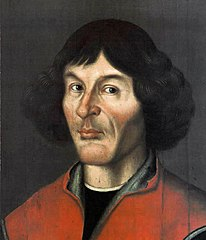
\includegraphics[width=8.3cm]{Nikolaus_Kopernikus} \caption{one column figure}\label{fig:unnamed-chunk-5}
\end{figure}

\subsubsection{TWO-COLUMN FIGURES}

\begin{figure}
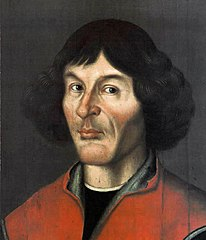
\includegraphics[width=12cm]{Nikolaus_Kopernikus} \caption{two column figure}\label{fig:unnamed-chunk-6}
\end{figure}

\subsection{TABLES}

You can add \LaTeX table in an R Markdown document to meet the template
requirements.

\subsubsection{ONE-COLUMN TABLE}

\begin{table}[t]
\caption{TEXT}
\begin{tabular}{l c r}
\tophline

a & b & c \\
\middlehline
1 & 2 & 3 \\

\bottomhline
\end{tabular}
\belowtable{Table Footnotes}
\end{table}

\subsubsection{TWO-COLUMN TABLE}

\begin{table*}[t]
\caption{TEXT}
\begin{tabular}{l c r}
\tophline

a & b & c \\
\middlehline
1 & 2 & 3 \\

\bottomhline
\end{tabular}
\belowtable{Table footnotes}
\end{table*}

\subsection{MATHEMATICAL EXPRESSIONS}

All papers typeset by Copernicus Publications follow the math
typesetting regulations given by the IUPAC Green Book (IUPAC:
Quantities, Units and Symbols in Physical Chemistry, 2nd Edn., Blackwell
Science, available at:
\url{http://old.iupac.org/publications/books/gbook/green_book_2ed.pdf},
1993).

Physical quantities/variables are typeset in italic font (t for time, T
for Temperature)

Indices which are not defined are typeset in italic font (x, y, z, a, b,
c)

Items/objects which are defined are typeset in roman font (Car A, Car B)

Descriptions/specifications which are defined by itself are typeset in
roman font (abs, rel, ref, tot, net, ice)

Abbreviations from 2 letters are typeset in roman font (RH, LAI)

Vectors are identified in bold italic font using \vec{x}

Matrices are identified in bold roman font

Multiplication signs are typeset using the LaTeX commands
\texttt{\textbackslash{}times} (for vector products, grids, and
exponential notations) or \texttt{\textbackslash{}cdot}

The character * should not be applied as mutliplication sign

\subsection{EQUATIONS}

\subsubsection{Single-row equation}

Unnumbered equations (i.e.~using \texttt{\$\$} and getting inline
preview in RStudio) are not supported by Copernicus.

\begin{equation}
1 \times 1 \cdot 1 = 42
\end{equation}

\begin{equation}
A = \pi r^2
\end{equation}

\begin{equation}
x=\frac{2b\pm\sqrt{b^{2}-4ac}}{2c}.  
\end{equation}

\subsubsection{Multiline equation}

\begin{align}
& 3 + 5 = 8\\
& 3 + 5 = 8\\
& 3 + 5 = 8
\end{align}

\subsection{MATRICES}

\[
\begin{matrix}
x & y & z\\
x & y & z\\
x & y & z\\
\end{matrix}
\]

\subsection{ALGORITHM/PROGRAMMING CODE}

If you want to use algorithms, you need to make sure yourself that the
\LaTeX packages \texttt{algorithms} and \texttt{algorithmicx} are
installed so that \texttt{algorithm.sty} respectively
\texttt{algorithmic.sty} can be loaded by the Copernicus template. Both
need to be available through your preferred \LaTeX{} distribution. With
TinyTeX (or TeX Live), you can do so by running
\texttt{tinytex::tlmgr\_install(c("algorithms",\ "algorithmicx"))}

\begin{verbatim}
## tlmgr update --all --self
\end{verbatim}

\begin{verbatim}
## tlmgr install algorithms algorithmicx
\end{verbatim}

Copernicus staff will no accept any additional packages from your LaTeX
source code, so please stick to these two acceptable packages. They are
needed to use the example below

\begin{algorithm}
\caption{Algorithm Caption}
\label{a1}
\begin{algorithmic}
\STATE $i\gets 10$
\IF {$i\geq 5$} 
        \STATE $i\gets i-1$
\ELSE
        \IF {$i\leq 3$}
                \STATE $i\gets i+2$
        \ENDIF
\ENDIF
\end{algorithmic}
\end{algorithm}

\subsection{CHEMICAL FORMULAS AND REACTIONS}

For formulas embedded in the text, please use
\texttt{\textbackslash{}chem\{\}}, e.g. \chem{A \rightarrow B}.

The reaction environment creates labels including the letter R, i.e.
(R1), (R2), etc.

\begin{itemize}
\item
  \texttt{\textbackslash{}rightarrow} should be used for normal
  (one-way) chemical reactions
\item
  \texttt{\textbackslash{}rightleftharpoons} should be used for
  equilibria
\item
  \texttt{\textbackslash{}leftrightarrow} should be used for resonance
  structures
\end{itemize}

\begin{reaction}
A \rightarrow B \\
\end{reaction}
\begin{reaction}
Coper \rightleftharpoons nicus \\
\end{reaction}
\begin{reaction}
Publi \leftrightarrow cations
\end{reaction}

\subsection{PHYSICAL UNITS}

Please use \texttt{\textbackslash{}unit\{\}} (allows to save the
math/\texttt{\$} environment) and apply the exponential notation, for
example \(3.14\,\unit{km\,h^{-1}}\) (using LaTeX mode:
\texttt{\textbackslash{}(\ 3.14\textbackslash{},\textbackslash{}unit\{...\}\ \textbackslash{})})
or \unit{0.872\,m\,s^{-1}} (using only
\texttt{\textbackslash{}unit\{0.872\textbackslash{},m\textbackslash{},s\^{}\{-1\}\}}).

\clearpage

\conclusions[Conclusions]

The conclusion goes here.






%%%%%%%%%%%%%%%%%%%%%%%%%%%%%%%%%%%%%%%%%%
%% optional

%%%%%%%%%%%%%%%%%%%%%%%%%%%%%%%%%%%%%%%%%%
\appendix
\section{Figures and tables in appendices}
\subsection{Option 1}

If you sorted all figures and tables into the sections of the text,
please also sort the appendix figures and appendix tables into the
respective appendix sections. They will be correctly named
automatically.

\subsection{Option 2}

If you put all figures after the reference list, please insert appendix
tables and figures after the normal tables and figures.

\texttt{\textbackslash{}appendixfigures} needs to be added in front of
appendix figures \texttt{\textbackslash{}appendixtables} needs to be
added in front of appendix tables

Please add \texttt{\textbackslash{}clearpage} between each table and/or
figure. Further guidelines on figures and tables can be found below.
Regarding figures and tables in appendices, the following two options
are possible depending on your general handling of figures and tables in
the manuscript environment: To rename them correctly to A1, A2, etc.,
please add the following commands in front of them:
\noappendix

%%%%%%%%%%%%%%%%%%%%%%%%%%%%%%%%%%%%%%%%%%
\authorcontribution{TIM and LAS: Conceptualization (lead); Data curation
(lead); Formal analysis (lead); Methodology (lead); Coding (lead);
Writing -- original draft (lead); Writing -- review and editing (lead).
SK: Conceptualization (lead); Formal analysis (supporting); Methodology
(supporting); Coding (supporting); Writing -- original draft
(supporting); Writing -- review and editing
(supporting).} %% optional section

%%%%%%%%%%%%%%%%%%%%%%%%%%%%%%%%%%%%%%%%%%
\competinginterests{The authors declare no competing
interests.} %% this section is mandatory even if you declare that no competing interests are present

%%%%%%%%%%%%%%%%%%%%%%%%%%%%%%%%%%%%%%%%%%

%%%%%%%%%%%%%%%%%%%%%%%%%%%%%%%%%%%%%%%%%%
\begin{acknowledgements}
Thanks to the rticles contributors!
\end{acknowledgements}

%% REFERENCES
%% DN: pre-configured to BibTeX for rticles

%% The reference list is compiled as follows:
%%
%% \begin{thebibliography}{}
%%
%% \bibitem[AUTHOR(YEAR)]{LABEL1}
%% REFERENCE 1
%%
%% \bibitem[AUTHOR(YEAR)]{LABEL2}
%% REFERENCE 2
%%
%% \end{thebibliography}

%% Since the Copernicus LaTeX package includes the BibTeX style file copernicus.bst,
%% authors experienced with BibTeX only have to include the following two lines:
%%
\bibliographystyle{copernicus}
\bibliography{../WeddellSea.bib}
%%
%% URLs and DOIs can be entered in your BibTeX file as:
%%
%% URL = {http://www.xyz.org/~jones/idx_g.htm}
%% DOI = {10.5194/xyz}


%% LITERATURE CITATIONS
%%
%% command                        & example result
%% \citet{jones90}|               & Jones et al. (1990)
%% \citep{jones90}|               & (Jones et al., 1990)
%% \citep{jones90,jones93}|       & (Jones et al., 1990, 1993)
%% \citep[p.~32]{jones90}|        & (Jones et al., 1990, p.~32)
%% \citep[e.g.,][]{jones90}|      & (e.g., Jones et al., 1990)
%% \citep[e.g.,][p.~32]{jones90}| & (e.g., Jones et al., 1990, p.~32)
%% \citeauthor{jones90}|          & Jones et al.
%% \citeyear{jones90}|            & 1990


\end{document}
